\Chapter{K-means klaszterezés}

\Section{Klaszterezés}

Ahhoz, hogy szürkeárnyalatos képeket megfelelően tudjunk kiszínezni, első lépésként meg kell határoznunk a kiszínezendő területeket. El kell döntenünk, hogy a kép mely részei tartoznak ugyan ahhoz a színárnyalathoz és melyek nem. Ezek alapján a dolgozat 2 fő részre bontható:
\begin{itemize}
\item képszegmentálás
\item szegmensek kiszínezése
\end{itemize}

A képszegmentálás célja az, hogy a képen lévő különböző célterületeket elkülönítse, a klaszterezés célja pedig az azonos tulajdonságokkal rendelkező objektumok közös kategóriába sorolása ahol az egy kategóriába tartozó objektumok egymáshoz hasonlóak, viszont különböznek a többi kategóriában lévő objektumoktól.

A két módszer célja lényegében megegyezik egymással. Ahhoz hogy a képből ki tudjuk nyerni a megfelelő szegmenseket, valamilyen klaszterezési eljárást kell alkalmaznunk.

A klaszterezési algoritmusokat a következő módon tudjuk csoportosítani \cite{clustering}:
\begin{itemize}
\item hierarchikus: a korábban létrehozott klaszterek felhasználásával találja meg az egymást követő klasztereket
    \begin{itemize}
    \item agglomeratív (bottom-up): minden egyes elemet különálló klaszterként kezel és azokat nagyobb klaszterekbe egyesíti
    \item osztó (top-down): a teljes halmazból indul ki és azt kisebb klaszterekre osztja
    \end{itemize}
\item particionáló: egyszerre határozza meg az összes klasztert
\item rács alapú: a teret véges számú cellára kvantálja amelyek egy rácsszerkezetet alkotnak, és ezeken hajtja végre a klaszterezést
\item modell alapú: megpróbálja az adatokat optimálisan ráilleszteni valamilyen matematikai modellre
\end{itemize}

A kutatások során az egyik legnépszerűbb particionáló klaszterezést használtam, a k-means klaszterezést.

\Section{K-means módszer}
A klaszterezés célja, hogy egy adathalmazt diszjunkt részhalmazokra (klaszterekre) ossza fel méghozzá úgy, hogy a klaszterezési kritérium optimális legyen. A legelterjedtebb klaszterezési kritérium az egyes adatpontok, és az azokat tartalmazó részhalmaz súlypontja (klaszterközéppont) közötti négyzetes Euklidészi távolságok összege. Ezt hívják klaszterezési hibának és ennek az optimalizálása a cél. \cite{kmeans}

A K-means algoritmus lokálisan optimális megoldásokat talál, figyelembe véve a klaszterezési hibát. Ez egy gyors, iteratív módszer aminek az algoritmusa a következő \cite{tomatoleaf}:
\begin{enumerate}
\item lépés: véletlenszerűen kiválaszt $K$ darab klaszterközéppontot
\item lépés: meghatározza az egyes pontok távolságát a középpontoktól valamilyen távolságfüggvény szerint, majd besorolja az egyes pontokat a hozzájuk legközelebbi klaszterközéppont kategóriájába
\item lépés: kiszámítja az egyes klaszterek számtani átlagát és az lesz az új klaszterközéppont
\item lépés: megnézi, hogy a klaszterközéppontok helyzetében történt-e változás:
    \begin{enumerate}
    \item ha igen, akkor megismétli az algoritmust a 2. lépéstől
    \item ha nem, akkor megáll az algoritmus, mivel megtalálta az optimális klasztereket
    \end{enumerate}
\end{enumerate}

A módszer nagy előnye hogy könnyen megvalósítható, viszont az algoritmusból láthatóak a módszer hátrányai is.

A végső klaszterezés a kezdeti klaszterközéppontok helyzetétől és a $K$ értékétől függ. A $K$ a klaszterek számát jelöli, és ezt az értéket nekünk kell meghatároznunk még a klaszterezési algoritmus futása előtt. Két K-means futási eredmény nagyban különbözhet, hiszen a középpontok kezdeti értéke véletlenszerű. Ahhoz, hogy ténylegesen az optimális eredményt kapjuk, érdemes az algoritmust többször futtatni.

Az optimális klaszterszám meghatározására több módszert is kipróbáltam, ezeket a \ref{optimal_cluster_number}. alfejezetben ismertetem.

A kutatásom során a \texttt{opencv-python} könyvtárban található K-means metódust használtam. Mivel a szegmentálás ez egyik fő eleme a kutatásomnak, így ezt is kiszerveztem az általam készített \texttt{commonmethods} könyvtárba \texttt{kmeans\_segmentation} néven. A következő kódrészletben látható az általam megírt algoritmus.
\begin{python}
def kmeans_segmentation(values, k):
    """
    Segmenting the given values using opencv-python's k-means method
    :param values: the values at which I want to perform segmentation
    :param k: the number of the clusters
    :return: the compactness, the labels and
        the centers from the k-means method
    """
    values = np.float32(values)

    criteria = \
        (cv2.TERM_CRITERIA_EPS + cv2.TERM_CRITERIA_MAX_ITER, 100, 0.2)

    compactness, labels, (centers) = cv2.kmeans(
        values,
        k,
        None,
        criteria,
        10,
        cv2.KMEANS_RANDOM_CENTERS)

    labels = labels.flatten()

    return compactness, labels, (centers)
\end{python}

Bemeneti paraméterként a szegmentálni kívánt értékeket és a klaszterek számát várja a metódus. Első lépésként átalakítom a kapott értékeket a \texttt{cv2.kemans} metódusnak megfelelő formátumra.

Maga a \texttt{cv2.kmeans} a következő paramétereket várja \cite{kmeans_opencv}:
\begin{itemize}
\item \texttt{samples}: Egy tömb amely \texttt{np.float32} típusú és a jellemzők külön oszlopokban helyezkednek el.
\item \texttt{nclusters(K)}: A klaszterek száma.
\item \texttt{bestLabels}: Bemeneti/kimeneti tömb amely minden mintához eltárolja a klaszterindexet.
\item \texttt{criteria}: Ez az iterációs kritérium. Ha ez teljesül, akkor az algoritmus megáll. A típusa tuple ami 3 paramétert tartalmaz:
    \begin{itemize}
    \item \texttt{type}: A leállási kritériumnak a típusa, 3 flagje (?) létezik:
        \begin{itemize}
        \item \texttt{cv.TERM\_CRITERIA\_EPS}: Akkor áll meg az algoritmus, ha elértük a kívánt pontosságot.
        \item \texttt{cv.TERM\_CRITERIA\_MAX\_ITER}: Akkor áll meg az algoritmus, ha elértük a maximális iterációk számát.
        \item \texttt{cv.TERM\_CRITERIA\_EPS} + \texttt{cv.TERM\_CRITERIA\_MAX\_ITER}: Akkor áll le az algoritmus, ha az előző két flag közül bármelyik bekövetkezik.
        \end{itemize}
    \item \texttt{max\_iter}: Az iterációk maximális száma.
    \item \texttt{epsilon}: Az elvárt pontosság.
    \end{itemize}
\item \texttt{attempts}: Azt adjuk meg, hogy hányszor fusson le az algoritmus különböző klasztereket eredményezve. A visszatérési érték a legoptimálisabb klaszter lesz.
\item \texttt{flags}: A kezdeti középpontok felvételének a módját tudjuk megadni. Általában 2 típusa van:
    \begin{itemize}
    \item \texttt{cv.KMEANS\_PP\_CENTERS}: Arthur és Vassilvitskii kmeans++ középpont inicializálási metódusát használva határozza meg a középpontokat.
    \item \texttt{cv.KMEANS\_RANDOM\_CENTERS}: Random határozza meg a középpontokat.
    \end{itemize}
\end{itemize}

A paramétereket úgy állítottam be hogy 10 alkalommal fusson le az algoritmus, és a klaszterek kezdő középpontját random határozza meg. Ezen kívül az algoritmus megáll ha eléri vagy a maximális iterációk számát ami 100, vagy a megfelelő pontosságot ami 0.2.

Ezeket a paramétereket a \cite{kmeans_opencv} dokumentáció alapján határoztam meg, egyedül a pontosságot, az \texttt{epsilon} értékét állítottam kisebbre mint a dokumentációban szereplő érték.

A k-means módszert kétféleképpen teszteltem le. Először csak a kép intenzitását vettem figyelembe, és az összes képpontot átadtam az algoritmusnak szegmentálásra. Ezek után feature vektorokat hoztam létre azzal a szándékkal, hogy textúra alapján végezzem a szegmentálást. A vizsgálatok eredménye a \ref{kmeans_intensity}. illetve a \ref{kmeans_texture} fejezetekben található.

\Section{Optimális klaszterszám meghatározása} \label{optimal_cluster_number}
Mint már említettem, a K-menas módszer egyik legfontosabb mozzanat a K érték meghatározása. Ez a fejezet néhány módszert mutat be, amellyel ezt meg tudjuk tenni.

Az optimális klaszterszám meghatározásához 4 módszert teszteltem le, ezeknek az eredménye a következő alfejezetekben található.
A módszereket a \cite{tomatoleaf} és a \cite{elbow} kutatások alapján választottam.

A módszereknél a klaszterekre bontás idejét nem veszem figyelembe, csak magának a módszernek a futási idejét.

\SubSection{Silhouette módszer}

A Silhouette index azt méri, hogy egy adott objektum mennyire hasonlít a saját klaszterében lévő objektumokhoz. Az értéke +1 és -1 között mozog. A nagyobb érték azt jelzi, hogy az objektum jól illeszkedik a saját klaszteréhez és rosszul illeszkedik a szomszédos klaszterekhez. Ha a legtöbb objektumnak pozitív az értéke akkor a klaszterezés megfelelő, ha sok objektumnak negatív akkor vagy túl sok, vagy túl kevés a klaszter.

A módszer a következő képlettel írható le:

\[ S(k)=\frac{1}{num} \sum_{i=1}^{num} \frac{b(i)-a(i)}{max\{a(i),b(i)\}} \quad \]

\noindent ahol
\begin{itemize}
\item $n$: a klaszterek száma
\item $num$: a pixelek száma
\item $a(i)$: az $i$ minta és az ugyanabban a klaszterben lévő többi minta közötti átlagos távolság
\item $b(i)$: az $i$ minta és az összes többi klaszter mintája közötti távolság minimális értéke
\end{itemize}
Ennek eredményeként megkapjuk a Silhouette pontszámot. Ha elvégezzük ezt a vizsgálatot különböző klaszterszámokra, akkor amelyiknek a pontszáma a legnagyobb, az lesz a legoptimálisabb klaszterszám. \cite{tomatoleaf}

Vizsgálataim során a \texttt{sklearn.metrics} csomagban található \texttt{silhouette\_score} módszert használtam a következő kódrészletben látható módon. Ez a metódus megtalálható az általam készített \texttt{commonmethods} csomagban.
\begin{python}
def silhouette_method(values, labels):
    """
    Calculating the Silhouette method for the given values with
    the given labels, and measuring time.
    :param values: in my case the pixel values from the k-means method
    :param labels: in my case the labels from the k-means method
    :return: the time of the calculation and
        the calculated Silhouette score
    """
    start = time.time()
    s_score = silhouette_score(values, labels)
    end = time.time()

    s_time = end-start

    return s_time, s_score
\end{python}
Mint látható, a metódus visszatér a módszer számítási idejével, mivel a vizsgálataim során a futási idők összevetése volt az egyik fő szempont. Ezen kívül visszaadja a kiszámított Silhouette pontszámot is, amit az általam megadott értékekből és a hozzájuk tartozó címkékből állít elő. Ezeket az értékeket a \texttt{kmeans\_segmentation} metódus eredményeként kapom.

A Silhouette módszer esetén azt tapasztaltam, hogy a futási ideje elég lassú. A \ref{fig:silhouette_runtime}. ábrán látható a módszer futási ideje különböző méretű képekre.

\begin{figure}[h]
\centering
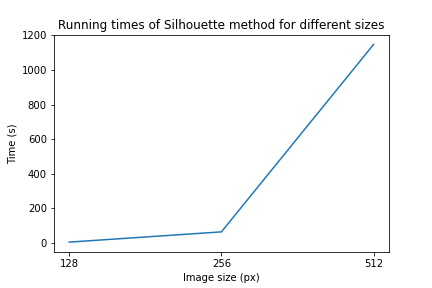
\includegraphics[scale=0.7]{images/silhouette_runtime.png}
\caption{A Silhouette módszer futási ideje különböző képméretekre.}
\label{fig:silhouette_runtime}
\end{figure}

Jól látható, hogy míg a 128px méretű képre pár másodperc alatt elvégzi a számítást, az 512px méretű képre már nagyságrendileg 20 percig számol.

\SubSection{Davies-Bouldin módszer}
A Davies-Bouldin index a klaszteren belüli szóródás összegének, és a klaszterek közötti szétválás arányának a függvénye. A célunk az hogy ezt az értéket minimalizáljuk, hiszen azt szeretnénk, hogy a klaszteren belüli szórás minimális, a klaszterek közötti elkülönülés pedig maximális legyen.

A módszer képlete a következő:

\[ DB(k)=\frac{1}{k} \sum_{i=1}^{K} max \left(\frac{W_i + W_j}{C_{ij}}\right)  \quad \]

\noindent ahol
\begin{itemize}
\item $K$: a klaszterek száma
\item $W_i$: a $C_i$ osztályba tartozó összes minta átlagos távolsága a klaszter középpontjától
\item $W_{j}$: a $C_i$ osztályba tartozó összes minta átlagos távolsága a $C_j$ osztály középpontjától
\item $C_{ij}$: a $C_i$ és $C_j$ osztályok középpontja közötti távolság
\end{itemize}
Ennek eredményeként megkapjuk a Davies-Bouldin pontszámot. Ha elvégezzük ezt a vizsgálatot különböző klaszterszámokra, akkor amelyiknek a pontszáma a legkisebb, az lesz a legoptimálisabb klaszterszám. \cite{tomatoleaf}

Ennek a módszernek a megvalósításához a \texttt{sklearn.metrics} csomagban található \texttt{davies\_bouldin\_score} metódust használtam. A következő kódrészletben látható, hogy a módszer megvalósítása ugyan arra a sémára épül, mint a \texttt{silhouette\_method}.

Ez a metódus is megtalálható az általam készített \texttt{commonmethods} csomagban.
\begin{python}
def davies_bouldin_method(values, labels):
    """
    Calculating the Davies-Bouldin method for the given values with
    the given labels, and measuring time.
    :param values: in my case the pixel values from the k-means method
    :param labels: in my case the labels from the k-means method
    :return: the time of the calculation and
        the calculated Davies-Bouldin score
    """
    start = time.time()
    db_score = davies_bouldin_score(values, labels)
    end = time.time()

    db_time = end-start

    return db_time, db_score
\end{python}

\SubSection{Calinski-Harabasz módszer}

A Calinski-Harabasz indexet belső klaszterérvényességi mérőszámként szokták használni, amely a létrehozott klasztereket osztályozza.

A módszer képlete a következő:

\begin{align*}
 CH(k) & =\frac{B(K)(N-K)}{W(K)(K-1)} \\
 B(K) & =\sum_{k=1}^{K}a_k \|\overline{x_k}-\overline{x}\|^2 \\
 W(K) & =\sum_{k=1}^{K}\sum_{C(j)=k}\|x_j-\overline{x_k}\|^2
\end{align*}

\noindent ahol
\begin{itemize}
\item $K$: a klaszterek száma
\item $N$: a minta száma
\item $B(K)$: a klaszterek közötti divergencia, más néven a klaszterek közötti kovariancia
\item $W(K)$: a klaszteren belüli divergencia, más néven a klaszteren belüli kovariancia
\end{itemize}

Minél nagyobb a $B(K)$ értéke, annál nagyobb a klaszterek közötti diszperzió mértéke. Minél kisebb a $W(K)$ értéke, annál szorosabb a kapcsolat a klaszteren belül. Minél nagyobb az arány, annál nagyobb a Calinski-Harabasz pontszám értéke, theát annál optimálisabb a klaszterszám. \cite{silhouette_calinski}

Ennek a módszernek a megvalósításához a \texttt{sklearn.metrics} csomagban található \texttt{calinski\_harabasz\_score} metódust használtam. A következő kódrészletben látható hogy, a módszer megvalósítása ugyan arra a sémára épül, mint a \texttt{silhouette\_method} és a \texttt{davies\_bouldin\_method}.

Ez a metódus is megtalálható az általam készített \texttt{commonmethods} csomagban.
\begin{python}
def calinski_harabasz_method(values, labels):
    """
    Calculating the Calinski-Harabasz method for the given values with
    the given labels, and measuring time.
    :param values: in my case the pixel values from the k-means method
    :param labels: in my case the labels from the k-means method
    :return: the time of the calculation and
        the calculated Calinski-Harabasz score
    """
    start = time.time()
    ch_score = calinski_harabasz_score(values, labels)
    end = time.time()

    ch_time = end-start
\end{python}

\SubSection{Elbow módszer}

Az Elbow módszer a variancia százalékos arányát vizsgálja a klaszterek számának függvényében. Azon az elven alapszik, hogy olyan klaszterszámot kell választanunk amelyhez ha hozzáadnánk akár csak egy klasztert is, akkor a modellünk már nem javulna számottevő mértékben.

Az első klaszterek sok információt adnak hozzá a modellhez, viszont egy bizonyos ponton a határnyereség drámaian lecsökken és szöget, vagyis könyököt képez a grafikonon (lásd. \ref{fig:elbow_grayscale}. ábra). Innen ered az "elbow" azaz "könyök" módszer elnevezés. Az a pont ahol ez a drámai csökkenés bekövetkezik, az lesz a megfelelő klaszterszám. A \ref{fig:elbow_grayscale}. ábrán ez a pont 2 klaszternél alakul ki, de érdemes lehet megvizsgálni a 3 klasztert is. \cite{elbow}

\begin{figure}[h]
\centering
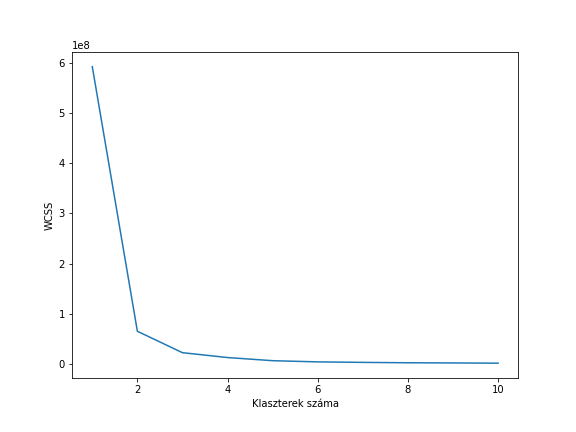
\includegraphics[scale=0.7]{images/elbow_grayscale.png}
\caption{Elbow módszer alkalmazása szürkeárnyalatos képre}
\label{fig:elbow_grayscale}
\end{figure}

Az Elbow metódushoz a \texttt{kmeans\_segmentation} által eredményként visszaadott \texttt{compactness} értékeket szükséges lementenünk különböző méretű klaszterekre ahogy az a következő kódrészletben látható.
\begin{python}
import commonmethods.image_modification as im

wcss = []   #within cluster sum of squares

for k in range(1, 11):
    compactness, _, _, _ = \
        im.kmeans_segmentation(resized_image, k)
    wcss.append(compactness)
\end{python}

Ha a \texttt{wcss} listát \texttt{plot} segítségével ábrázoljuk, meg is kaptuk az Elbow grafikonunkat pont úgy, mint ahogy a \ref{fig:elbow_grayscale}. ábrán szerepel.

Ennél a módszernél külön számítást nem kell végeznünk, így futási ideje igazából csak maga a kirajzolás.

Összességében a módszer gyors, viszont nem mindig ad egyértelmű eredményt és a töréspont automatizált meghatározása sem egy egyszerű feladat. Vizuális ábrázolásra és kézi ellenőrzésre viszont megfelelő, így főként én is erre a célra használtam.

\SubSection{Összegzés}

A módszerek vizsgálata során hamar kiderült, hogy a Silhouette módszer futási ideje számottevően nagyobb a többi módszerétől. Az eredmények összehasonlítását a \ref{tab:size_runtimes}. táblázat tartalmazza. Mivel az Elbow módszer nem egyértelmű és főként vizuális megerősítésként szolgál, így ezt a módszert kihagytam a további elemzésekből.

\begin{table}[h]
\centering
\caption{Futási idők átlaga különböző módszerek esetén}
\label{tab:size_runtimes}
\medskip
\begin{tabular}{|l|c|c|c|c|}
\cline{2-5}
 \multicolumn{1}{c|}{} & \multicolumn{4}{c|}{Kép mérete} \\
 \hline
 Módszer & 64px & 128px & 256px & 512px \\
\hline
Silhouette módszer & 0.2684s & 4.4029s & 68.0697s & 1183.2937s \\
Davies-Bouldin módszer & 0.0071s & 0.0042s & 0.0096s & 0.0274s \\
Calinski-Harabasz módszer & 0.0031s & 0.001s & 0.0028s & 0.0120s \\
\hline
\end{tabular}
\end{table}

A táblázat jól szemlélteti, hogy a Silhouette módszer futási ideje már a legkisebb képméretre is majdnem negyveszerese a másik két módszer futási idejének.

Mivel a klaszterek számának növelésével a feldolgozandó adathalmaz nem változik, így a klaszterek száma nem befolyásolja a módszerek futási idejét. Erre bizonyítékként szolgál a \ref{tab:cluster_runtimes}. táblázat amely különböző klaszterszám esetén mutatja be az átlagos futási időket. Jól látható hogy nem növekszik, sőt valahol csökken a magasabb klaszterszám esetén a futási idő.

\begin{table}[h]
\centering
\caption{Futási idők átlaga különböző klaszterszámok és módszerek esetén, 256px képméretre}
\label{tab:cluster_runtimes}
\medskip
\begin{tabular}{|l|c|c|c|}
\cline{2-4}
 \multicolumn{1}{c|}{} & \multicolumn{3}{c|}{Klaszterek száma} \\
 \hline
 Módszer & 2 & 4 & 8 \\
\hline
Silhouette módszer & 63.1462s & 63.1254s & 62.2278s \\
Davies-Bouldin módszer & 0.0060s & 0.0083s & 0.0064s \\
Calinski-Harabasz módszer & 0.0026s & 0.0024s & 0.0028s \\
\hline
\end{tabular}
\end{table}

Természetesen a K-means metódus lassabban határozza meg a klasztereket nagyobb klaszterszám esetén, így a nagyobb klaszterszám magának a programnak a futási idejét befolyásolja.

A futási idők mellett a módszerek jóságát is megvizsgáltam mind színes, mind szürkeárnyalatos képek esetén. Ennek a vizsgálatnak az eredményét a \ref{tab:cluster_result}. táblázatban foglaltam össze.

A módszereket minden képméretre több alkalommal is lefuttattam, ezekből a futások alkalmával kapott összes klaszterszámot megjelenítettem. Jól látható, hogy a Silhouette és a Davies-Bouldin módszer minden képméretre, minden futási alkalommal ugyanazt az eredményt szolgáltatta, és a két módszer eredményei megegyeznek.

Ezzel szemben a Calinski-Harabasz módszer eredménye eltér a másik 2 módszer eredményétől, és a különböző képméretekre más-más klaszterszámmal szolgált. Emelett még az is látható hogy egy azon képméret esetén, például a 64px méretű színes képnél több futás alkalmával más-más klaszterszámot adott eredményül.

\begin{table}[h]
\centering
\caption{Meghatározott klaszterszám különböző képméretek és módszerek esetén}
\label{tab:cluster_result}
\medskip
\begin{tabular}{|l|c|c|c|c|c|c|}
\cline{2-7}
 \multicolumn{1}{c|}{} & \multicolumn{6}{c|}{Kép mérete} \\
 \hline
 \multirow{2}{*}{Módszer} & \multicolumn{2}{c|}{64px} & \multicolumn{2}{c|}{126px} & \multicolumn{2}{c|}{256px} \\
 \cline{2-7}
 & Szürke & Színes & Szürke & Színes & Szürke & Színes  \\
\hline
Silhouette módszer & 2 & 3 & 2 & 3 & 2 & 3 \\
Davies-Bouldin módszer & 2 & 3 & 2 & 3 & 2 & 3 \\
Calinski-Harabasz módszer & 10 & 8,10 & 9,10 & 10 & 9 & 8,9 \\
\hline
\end{tabular}
\end{table}

Elvégeztem az Elbow módszert is a színes képre, ennek az eredménye a \ref{fig:elbow_rgb}. ábrán látható. A szürkeárnyalatos változatát a \ref{fig:elbow_grayscale}. ábra tartalmazza, ezt használtam fel példának az Elbow módszer bemutatásakor. Látható, hogy mind a két esetben a 2 és 3 klaszternél található meg törés a grafikonon, tehát az Elbow módszer is ezeket a klaszterszámokat javasolja.

\begin{figure}[h]
\centering
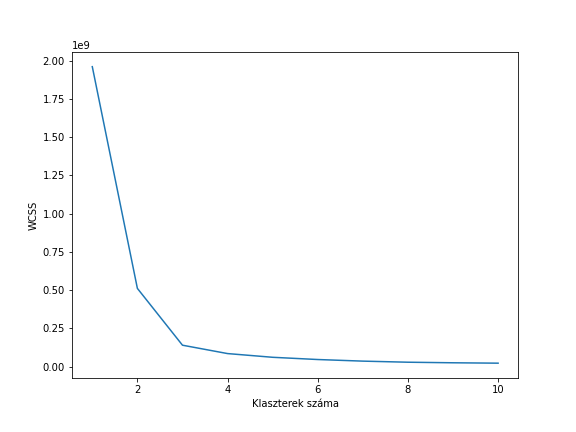
\includegraphics[scale=0.7]{images/elbow_rgb.png}
\caption{Elbow módszer alkalmazása színes képre}
\label{fig:elbow_rgb}
\end{figure}

A Módszerek által megadott klaszterszámokkal elvégeztem a klaszterezést, az eredmény a \ref{fig:kmeans_optimal_pictures}. ábrán látható.

\begin{figure}[h]
\centering
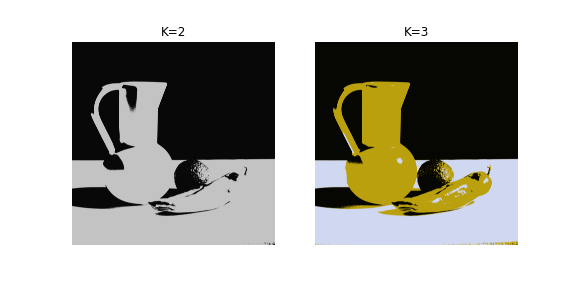
\includegraphics[scale=0.7]{images/kmeans_optimal_pictures.png}
\caption{K-means klaszterezés a módszerek által megadott optimális klaszterszámmal}
\label{fig:kmeans_optimal_pictures}
\end{figure}

Összegezve a vizsgálatokat ki lehet jelenteni, hogy a legjobb módszer az optimális klaszterszám meghatározására a vizsgáltak közül az a Davies-Bouldin módszer.

A Silhouette-módszer igaz hogy pontos, de a futási ideje nagyon magas. Ha egészen kis méretű képeket használunk akkor talán még alkalmazható, de nagyobb képek esetén nagyon megnöveli a program futási idejét.

A Calinski-Harabasz módszer futási ideje sok esetben jobb volt, mint a Davies-Bouldin módszeré, viszont a klaszterszám meghatározása nagyon pontatlan. Egyszer sem szolgáltatta azt az eredményt amit a másik három módszerből kaptam.

\Section{Klaszterezés intenzitás alapján} \label{kmeans_intensity}

Az intenzitás alapú szegmentálás során nem volt másra szükségem, csak a kép pixeleinek az értékére. A szürkeárnyalatos kép pixeleit egy $n\times1$ méretű, a színes képek pixeleit pedig egy $n\times3$ méretű tömbbé alakítottam át. Erre a \texttt{numpy} csomagban található \texttt{reshape} metódust használtam a következő kódrészletben látható módon.
\begin{python}
#grayscale image
grayscale_pixel_values = grayscale_image.reshape((-1, 1))

#rgb image
rgb_pixel_values = rgb_image.reshape((-1, 3))
\end{python}

A megkapott értékeket adtam át a \texttt{kmeans\_segmentation} metódusnak.

A szegmentálás eredményei különböző számú klaszterekre a \ref{fig:kmenas_grayscale}. ábrán látható szürkeárnyalatos képek esetén, és a \ref{fig:kmenas_rgb}. ábrán látható színes képek esetén. Mind a két esetben 2, 4, és 8 értékeket állítottam be a klaszterek számának.

A szegementált képeket a \texttt{kmeans\_segmentation} által előállított \texttt{labels} és \texttt{centers} értékek segítségével rajzolom ki. Az egy kategóriába tartozó pixeleket kiszínezem a kategóriájuk középpontjával megegyező színnel a következő kódrészletben látható módon.

\begin{python}
centers = np.uint8(centers)
segmented_image = centers[labels.flatten()]
segmented_image = segmented_image.reshape(image.shape)
\end{python}

Először a középpontok értékét \texttt{np.float32} típusról átalakítom integer típusra, majd a \texttt{labels} értékek alapján létrehozom a szegmentált kép pixeleit tartalmazó tömböt. Ez a tömb egy dimenziós lesz, így kirajzolás előtt átalakítom az eredeti képpel megegyező formátumra.

\begin{figure}[h]
\centering
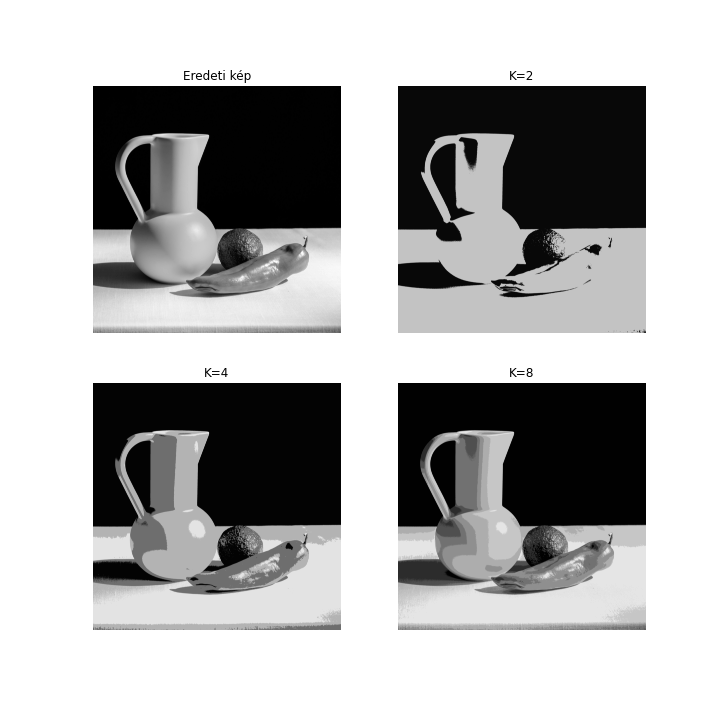
\includegraphics[scale=0.6]{images/kmeans_grayscale.png}
\caption{K-means módszer futási eredménye szürkeárnyalatos kép esetén, különböző klaszterszámokra}
\label{fig:kmenas_grayscale}
\end{figure}

\begin{figure}[h]
\centering
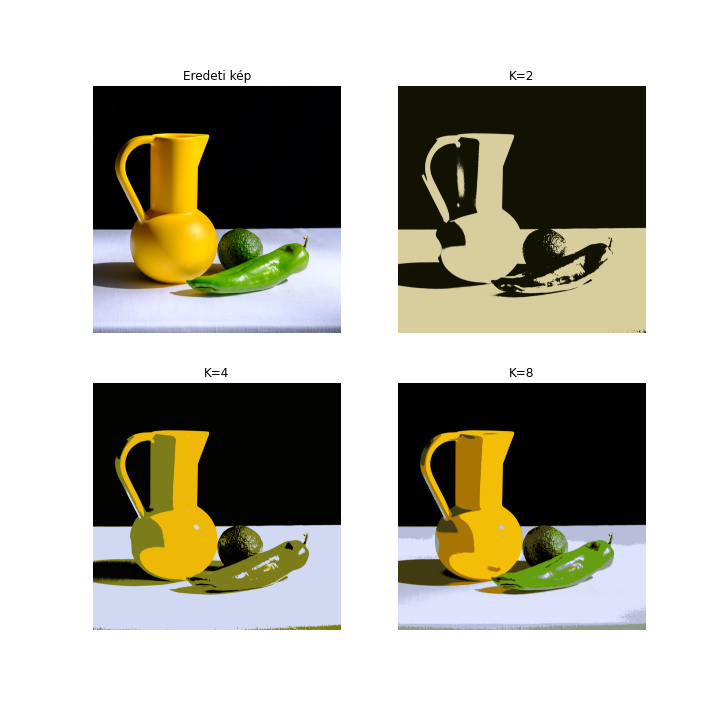
\includegraphics[scale=0.6]{images/kmeans_rgb.png}
\caption{K-means módszer futási eredménye színes kép esetén, különböző klaszterszámokra}
\label{fig:kmenas_rgb}
\end{figure}

A módszer vizsgálata során kitértem a futási időre is. Logikusan következik, hogy a képek méretének növelésével, vagy a klaszterek számának növelésével a módszer futási ideje is növekszik. A \ref{fig:kmenas_runtime_cluster}. és a \ref{fig:kmenas_runtime_size}. ábrákon található ezeknek a vizsgálatoknak az eredménye.

Jól látható, hogy a klaszterek számának növelésével a futási idő nem minden alkalommal növekszik, viszont a képek méretének növelésével a futási idő növekedése folyamatos. Emellett az is megfigyelhető, hogy sem a legnagyobb vizsgált klaszterszám (10), sem a legnagyobb vizsgált képméret (768px) esetén nem éri el a futási idő a 0.5 másodpercet, tehát az algoritmus futási ideje még ezekben az esetekben is gyors.

\begin{figure}[h]
\centering
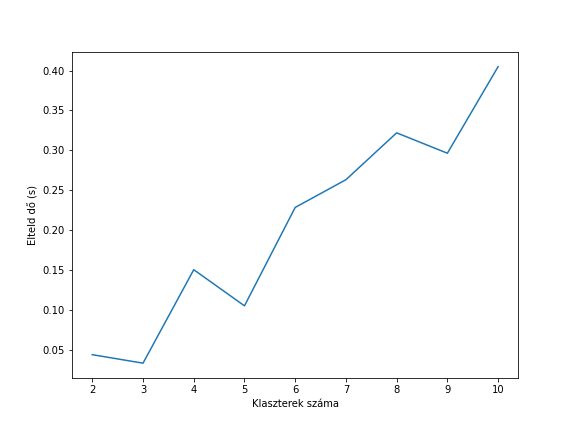
\includegraphics[scale=0.7]{images/kmeans_runtime_cluster.png}
\caption{K-means módszer futási ideje különböző klaszterszámokra}
\label{fig:kmenas_runtime_cluster}
\end{figure}

\begin{figure}[h]
\centering
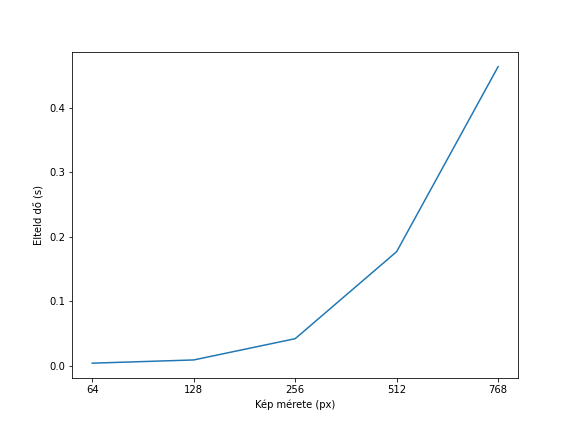
\includegraphics[scale=0.7]{images/kmeans_runtime_size.png}
\caption{K-means módszer futási ideje különböző méretű képekre}
\label{fig:kmenas_runtime_size}
\end{figure}

A futási idők után megvizsgáltam, hogy vajon különböző méretű képekre mennyire pontos a klaszterezés. A klaszterek számának 4-et adtam meg, a klaszterezést pedig elvégeztem 64px, 128px, 256px és 512px méretű képekre. A futási eredményeket a \ref{fig:kmenas_picture_sizes}. ábra tartalmazza.

Egyértelműen látszik, hogy már a legkisebb, 64px méretű képen is ugyanazokat a klasztereket találja meg mint a legnagyobb, 512px méretű képen.

\begin{figure}[h]
\centering
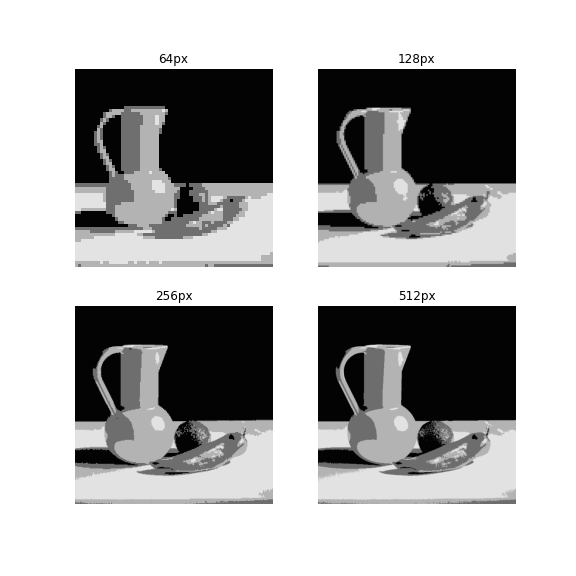
\includegraphics[scale=0.7]{images/kmeans_picture_sizes.png}
\caption{K-means módszer futási eredménye különböző méretű képekre}
\label{fig:kmenas_picture_sizes}
\end{figure}

\Section{Klaszterezés textúra alapján} \label{kmeans_texture}

Az intenzitás alapú klaszterezés során az objektumokat egymástól nem igazán lehetett megkülönböztetni, így másik módszert próbáltam alkalmazni.

A textúra alapú klaszterezés során úgynevezett feature vektorokat készítettem és ezeket adtam át a \texttt{kmeans\_segmentation} metódusomnak. A feature vektor egy $n\times px^2$ méretű tömb, ami $n$ darab az eredeti képből kivágott $px \times px$ méretű ablakot tartalmaz. Ezek az ablakok tartalmazzák a különböző textúrákat. A szegmentálás során a K-means módszer megpróbálja megtalálni az egymáshoz legjobban hasonlító ablakokat, vagyis textúrákat.

Egy ablak kinyerését a következő kódrészletben látható \texttt{get\_window} metódus végzi el.
\begin{python}
import numpy as np

def get_window(image, row_number, column_number, px):
    """
    Method for getting the px x px sized window from the image.
    :param image: the image that I want to get the window from
    :param row_number: the row where the window left corner pixel
        should start
    :param column_number: the column where the window left corner pixel
        should start
    :param px: the width and height of the window
    :return: the px x px sized window from the image
    """
    window = np.zeros((px, px))

    for i in range(0, px):
        column = np.zeros((px))
        for j in range(0, px):
            column[j] = image[row_number+i][column_number+j]
        window[i] = column

    return window
\end{python}

A függvény bemenetként a képet, az ablak méretét, és az ablak bal felső pixelének az $x, y$ koordinátáit várja \texttt{column\_number} és \texttt{row\_number} néven.

Első lépésként létrehozok egy $px \times px$ méretű tömböt amit feltöltök nullákkal, majd indítok két egymásba ágyazott for ciklust nullától $px$ méretéig. A külső ciklusban az oszlopokat hozom létre, majd a belső ciklussal végig haladok az oszlopban található pixelek értékein, és lementem őket. Az így kapott oszlopokat összefűzve megkapom a képemből kinyert ablakot.

A függvény által meghatározott ablakokra példa a \ref{fig:window_example}. ábrán található. A \texttt{px} értékének 15-öt állítottam be, az ablakok kezdőértékei pedig a képek tetején szerepelnek. Az eredeti kép, az 5.jpg látható a bal felső ábrán. Az ablakok a képnek a különböző textúráit mutatják be, mindegyik textúra felett megtalálható annak az objektumnak a neve amiről származik. Megfigyelhető hogy amíg a háttér, az avokádó, és a terítő textúrája elég egyedi, addig a kancsó és a paprika textúrája nagyon hasonló egymáshoz. Az ő esetükben szükség lehet az ablakokon kívül más értékekre is (például az intenzitásukra), ami alapján a szegmentálás során meg lehet őket különböztetni.

\begin{figure}[h]
\centering
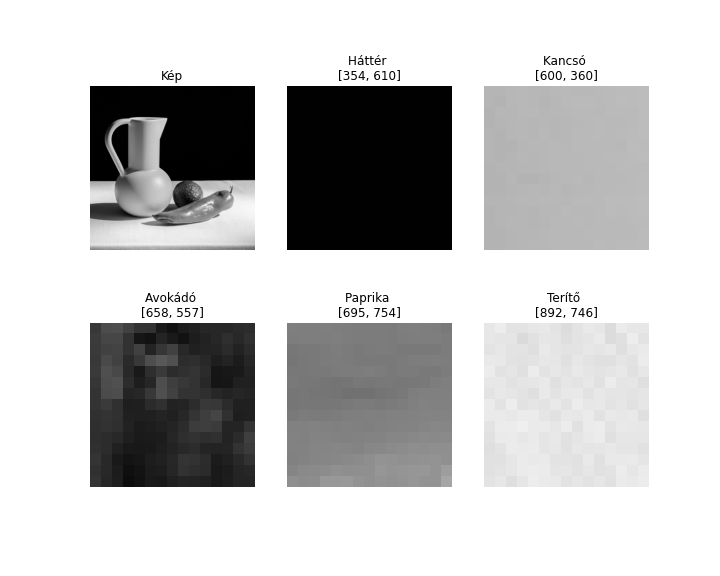
\includegraphics[scale=0.6]{images/window_example.png}
\caption{$15px\times 15px$ méretű minta ablakok a vizsgált képen található különböző textúrákról.}
\label{fig:window_example}
\end{figure}

Ahhoz, hogy a teljes képet szegmentálni tudjam, szükségem van több ilyen $px \times px$ méretű ablakra. Hogy minél nagyobb valószínűséggel lefedjem a képen található összes textúrát, az ablakok helyzetét random határozom meg. Készítettem egy metódust \texttt{get\_window\_values} néven, ami a következő kódrészletben található.
\begin{python}
import numpy as np

def get_window_values(image, window_quantity, px):
    """
    Method for getting random windows from the image,
    stacked in one vector.
    The resulted vector size will be window_quantity x px*px.
    :param image: the image that i want to get the random windows from
    :param window_quantity: the amount of windows that i want to get
    :param px: the width and height of the windows
    :return: the result, which is the vector created from the windows,
        and the pixels, an array that contains the start pixels
        of the windows
    """
    height = image.shape[0]
    width = image.shape[1]

    pixels = np.zeros((window_quantity, 2))

    #get random window start pixels
    x = np.random.randint(0, height-px, window_quantity)
    y = np.random.randint(0, width-px, window_quantity)

    for i in range(window_quantity):
        window = get_window(image, x[i], y[i], px)
        window = window.reshape((1, -1))
        pixels[i] = [x[i], y[i]] #saving the start pixels of the windows

        if i == 0:
            result = np.array(window)
        else:
            result = np.vstack([result, window])

    return result, pixels
\end{python}

A függvény bemeneti paraméterként az ablakok számát és a méretét, ezen kívül azt a képet várja, amin az ablakokat szeretném meghatározni.

Első lépésként létrehozok egy tömböt \texttt{pixels} néven, amiben az ablakok kezdeti pixeleit fogom eltárolni. Ezután a \texttt{numpy} csomag \texttt{random.randint} metódusa segítségével létrehozok \texttt{window\_quantity} mennyiségű, 0 és a kép mérete-px közötti integer számokat. 2 listát kapok, az egyikből kapom meg az $x$, a másikból az $y$ koordinátáit az ablakok kezdő pixeleinek. Egy for ciklus segítségével létrehozok \texttt{window\_quantity} darabszámú ablakot a fentebb említett \texttt{get\_window} függvény segítségével. A megkapott ablakokat átalakítom 1 dimenziós tömbbé, majd hozzáadom a \texttt{result} listához.

Eredményül egy $\texttt{window\_quantity} \times px^2$ méretű tömböt kapok. Ez lesz az a feature vektor, amit átadok a \texttt{kmeans\_segmentation} metódusomnak szegmentálásra.

A szegmentálás eredményeként minden ablakra kapok egy címke értéket. Annak érdekében hogy a pixeleket a megfelelő címke szerint tudjam egyszerűen kiszínezni, készítettem egy \texttt{get\_label\_map} nevű metódust amit a következő kódrészlet tartalmaz.

\begin{python}
def get_label_map(height, width, pixels, labels, px):
    """
    Method for getting the label to each pixel of the windows.
    :param height: the height of the image that contains the windows
    :param width: the width of the image that contains the windows
    :param pixels: the starting pixels of the previously
        calculated windows
    :param px: the width and height of the windows
    :return: an array in the shape of the image,
        the values are -1 where the pixel is not segmented,
        the labels elswhere
    """
    label_map = np.full((height, width), -1)

    for i in range(len(pixels)):
        for j in range(0, px):
            for k in range(0, px):
                label_map[int(pixels[i][0]+j)][int(pixels[i][1]+k)] =\
                    labels[i]

    return label_map
\end{python}

A függvény bemeneti paraméterként az eredeti kép méreteit, az ablakok méretét és kezdő pixeleit, ezen kívül a címkéket várja. Első lépésként létrehozok egy tömböt, ami ugyanolyan formájú mint maga a kép, és feltöltöm minden értékét -1-gyel. Ehhez a \texttt{numpy} csomag \texttt{full} függvényét használom. A -1 fogja jelezni, hogy egy pixel még nem kapott címkét. Ezután indítok egy for ciklust ami végig halad az ablakok kezdő pixelein. A kezdő értékektől indulva bejárom a $px \times px$ méretű ablakot, így megkapva az ablak összes pixelét, és minden pixelhez az ablakhoz kapott címkét rendelem hozzá. Eredményként kapok egy olyan térképet, ami a szegmentált pixelnél a címkét, a még nem szegmentált pixelnél pedig -1-et tartalmaz.

A megkapott szegmensek kirajzolása érdekében készítettem egy \texttt{color\_image} metódust ami a következő kódrészletben látható.

\begin{python}
import cv2
import numpy as np

def color_image(image, label_map):
    """
    Method for colorizing the image based on the label_map.
    :param image: the image which I want to colorize
    :param label_map: the map of the labels, I choose the color
        of the pixels by the label given to the pixel
    :return: the colorized image
    """
    height = image.shape[0]
    width = image.shape[1]

    colored_image = cv2.cvtColor(image, cv2.COLOR_GRAY2RGB)

    colors = np.array([
        [0, 0, 255],   #blue
        [255, 0, 0],   #red
        [255, 255, 0], #yellow
        [0, 255, 0],   #lime
        [0, 255, 255], #cyan
        [255, 150, 0]  #orange
    ])

    for i in range(height):
        for j in range(width):
            if(label_map[i][j] != -1):
                colored_image[i][j] = colors[label_map[i][j]]

    return colored_image
\end{python}

A metódus bemeneti paraméterként azt a képet várja amit színezi szeretnénk, emellett a képpel megegyező formátumú címke tömböt. Meghatározzuk a kép magasságát és szélességét, hogy for ciklussal végig tudjunk iterálni rajta. Ezután a \texttt{cv2} csomag \texttt{cvtColor} függvényével a paraméterként kapott képet átalakítom RGB formátumúra. Ez azt jelenti, hogy a pixelekhez tartozó eddigi 1 érték helyett hozzárendelünk egy 3 értékű tömböt, ami háromszor tartalmazza ugyanazt az értéket. Ettől kezdve színeket tudunk hozzárendelni a pixelekhez.

Egy \texttt{colors} nevezetű tömbbe lementettem 6 szín RGB kódját. A pixel címke értéke 0 és k között lehet, így a színeknél a maximális klaszterszám (jelen esetben) 6. Minden pixelt helyettesítek a \texttt{colors} listából a címke értékével megegyező elemmel. Például ha a pixel címkéje 0, akkor a colors[0]. elemét fogja megkapni. Ennek eredményeként az egy szegmensbe tartozó pixelek ugyanazt a színt fogják megkapni.

Visszatérési értéke a függvénynek a színekkel ellátott kép. Ebben az esetben még árnyalatokat nem veszünk figyelembe, a színezés célja a szegmensek szemléltetése.

A \ref{fig:window_colorized}. ábrán az eddig említett metódusok felhasználásával készített kép látható. A képhez beolvasás után 5000 darab, $15\times15$ px méretű ablakot generáltam a \texttt{get\_window\_values} függvénnyel, majd szegmentáltam a kapott értékeket $k=5$ paraméterrel a \texttt{kmeans\_segmentation} felhasználásával. Ezek után meghatároztam a címke térképet a \texttt{get\_label\_map} függvénnyel, végül kiszíneztem a képet az imént említett \texttt{color\_image} metódussal.

\begin{figure}[h]
\centering
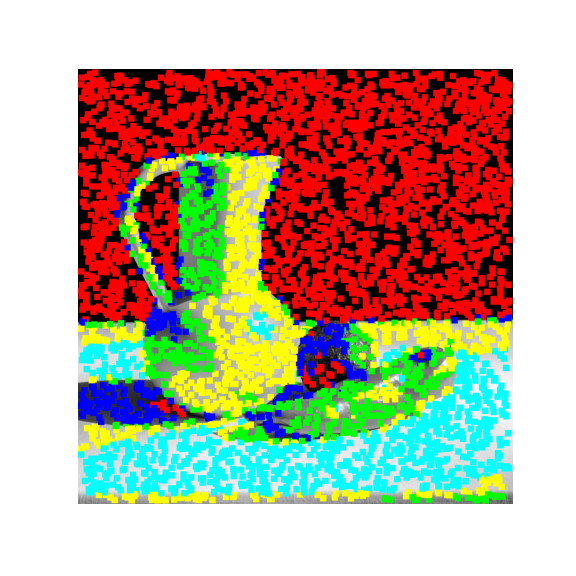
\includegraphics[scale=0.6]{images/window_colorized.png}
\caption{5000 darab, $15 \times 15$ px méretű ablak szegmentálása és megjelenítése az eredeti képen.}
\label{fig:window_colorized}
\end{figure}

Az ablakok szegmentálása után a kép többi részét is be kell osztanunk a kialakult szegmensekbe, ehhez valamilyen osztályozási módszerre van szükségünk.

\SubSection{Osztályozás}

Az osztályozási problémák célja azon jellemzők azonosítása amelyek jelzik, hogy az egyes esetek melyik csoportba tartoznak. A jellemzőkből álló minta felhasználható a meglévő adatok vizsgálatára és az új adatok viselkedésének előrejelzésére is. Az osztályozási modelleket már meglévő, osztályozott adatok vizsgálatával hozzák létre.

Az egyik legegyszerűbb osztályozási módszer a K-Nearest Neighbor (KNN). A mintafelismerésben a KNN algoritmus a tulajdonságtérben található legközelebbi gyakorló példák alapján osztályozza az objektumokat. A KNN egyfajta példányalapú tanulás, vagy lusta tanulás, ahol a függvényt csak lokálisan közelítjük, és minden számítást elhalasztunk az osztályozásig. Ez a módszer megtartja a teljes tanítóhalmazt a tanulás során, és minden egyes lekérdezésnél veszi az új elemhez legközelebb levő K elemet, megvizsgálja az elemek osztályát és amelyik osztályból a legtöbb található a K elem között, az lesz az új objektum osztálya is.

A KNN-osztályozó teljesítményét elsősorban a K értéke és az alkalmazott távolsági metrika határozza meg. Ha K nagyon kicsi, a lokális becslés az adatok ritkasága és a zajos, kétértelmű vagy rosszul címkézett pontok miatt általában nagyon gyenge lesz. A becslés további simítása érdekében növelhetjük K-t, és figyelembe vehetünk egy nagy régiót a lekérdezés körül. Sajnos a nagy K érték sem a legmegfelelőbb, mivel az osztályozási teljesítményt rontják a más osztályokból származó kiugró értékek. \cite{knn}

Hasonlóan a K-means módszerhez, itt is az egyik legfontosabb lépés a megfelelő K érték meghatározása. Az ökölszabály az az, hogy a tanító halmaz elemszámának a gyökét adják meg a K értékének. Mivel ez nem feltétlen a legoptimálisabb érték, így én több K értéket is megvizsgálok, és a legjobb pontossággal rendelkezőt választom. A K meghatározására létrehoztam egy \texttt{determine\_K\_value} nevű függvényt ami a következő kódrészletben látható.
\begin{python}
import math
import numpy as np
from sklearn.neighbors import KNeighborsClassifier
from sklearn.model_selection import train_test_split

def determine_K_value(values, labels):
    """
    Method for determining the best K value for KNN method.
    :param values: the values that I want to use to teach the modell
    :param labels: the labels to the values
    :return: the best K value, the training values and labels
        for teaching the model
    """
    values_train, values_test, labels_train, labels_test =\
        train_test_split(
            values,
            labels,
            stratify = labels,
            train_size = 0.8)

    root =  int(math.sqrt(values_train.shape[0]))

    neighbors = np.arange(root-10, root+10)

    train_accuracy = np.empty(len(neighbors))
    test_accuracy = np.empty(len(neighbors))

    for i, k in enumerate(neighbors):
        knn_model = KNeighborsClassifier(n_neighbors=k)
        knn_model.fit(values_train, labels_train)

        train_accuracy[i] = knn_model.score(values_train, labels_train)
        test_accuracy[i] = knn_model.score(values_test, labels_test)

    max_train = max(train_accuracy)
    max_train_k =\
        neighbors[np.where(train_accuracy == max(train_accuracy))]
    max_test = max(train_accuracy)
    max_test_k =\
        neighbors[np.where(test_accuracy == max(test_accuracy))]

    chosen_k = -1
    if(len(max_test_k) > 1):
        for k in max_test_k:
            if(k in max_train_k):
                chosen_k = k
                break
    else:
        chosen_k = max_test_k[0]

    if(chosen_k == -1):
        chosen_k = np.random.choice(max_test_k)

    return chosen_k, values_train, labels_train
\end{python}

A modellem létrehozására és az adathalmazom formálásra a \texttt{sklearn} könyvtárban található függvényeket használom. A modellem betanításához szükségem van egy, már szegmentált mintahalmazra, így első lépésként meghatározok ablakokat amiket átadok a \texttt{kmeans\_segmentation} metódusnak. Az értékeket, és a kapott címkéket adom át a \texttt{determine\_K\_value} függvénynek, ami \texttt{values} illetve \texttt{labels} paraméterként várja őket.

Szeretném tesztelni a modell hatékonyságát, így első lépésként fel kell osztanom az adathalmazomat tanító és tesztelő részhalmazokra.

A felbontáshoz a \texttt{sklearn.model\_selection} csomagból a \texttt{train\_test\_split} függvényt használom. A halmazt 80\%-20\% arányban osztom fel tanító és teszt részhalmazra, ezen kívül megadom, hogy a felbontás során ugyanannyi százalékban tartalmazzon mind a két halmaz elemeket az egyes címkékből.

Az adatok szétválasztása után létrehozom azt a listát, ami a lehetséges K elemeket fogja tartalmazni. Ehhez meghatározom a tanító halmazom elemszámának gyökét, és ehhez mérten a tőle $\pm 10$ intervallumban levő értékeket vizsgálom.

Ezután egy for ciklussal végig iterálok a meghatározott K értékeken. A cikluson belül létrehozom a modellemet a \texttt{sklearn.neighbors} csomag \texttt{KNeighborsClassifier} függvényével az éppen vizsgált K érték megadásával. A modell definiálása után a tanító adatokkal betanítom, majd a teszt adatokkal megvizsgálom a modell pontosságát. Mint látható, két már előre definiált tömbbe lementem a különböző K értékek tesztelési pontosságát a modell \texttt{score} függvényének a segítségével. A kapott pontossági értékeket grafikonon szemléletesen lehet ábrázolni, erre példa a \ref{fig:knn_accuracy}. ábrán látható. Megfigyelhető, hogy a modell pontossága 95\% felett található minden K értékre.

\begin{figure}[h]
\centering
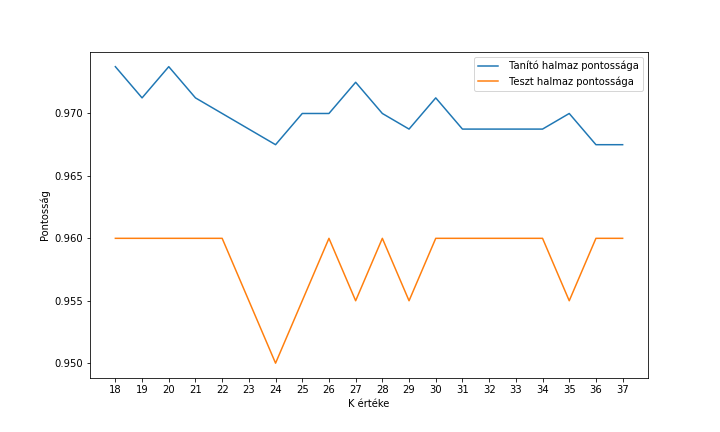
\includegraphics[scale=0.6]{images/knn_accuracy.png}
\caption{KNN modell pontosságát szemléltető grafikon.}
\label{fig:knn_accuracy}
\end{figure}

Mivel több érték is előfordulhat ami a teszt halmazra maximum pontosságot eredményez, így a megfelelő K értékét a tanító halmaz legjobb eredményeinek a figyelembevételével határozom meg. Amennyiben több a teszt halmazban található elem is elérte a maximum pontosságot, akkor megvizsgálom, hogy a tanító halmazban is maximális pontosságot ért-e el az adott K érték. Ha igen, akkor az első ilyen esetnél megállok és az lesz a választott K. Ha nincs ilyen, akkor random választok a legjobb teszt halmaz eredményeiből. Természetesen ha csak 1 K érték érte el a maximális pontosságot a teszt halmazon, akkor az lesz a választott K érték.

A \ref{fig:knn_accuracy}. ábra esetében a választott K érték a 18 lenne, mivel a teszt és tanító halmaz pontossága is maximális az adott helyen. Ez fenn áll a K=20 helyen is, viszont az algoritmusom az első találatnál megáll, hiszen mind a kettő K érték ugyan olyan eredményt produkál.

Miután meghatároztuk a K megfelelő értékét létre kell hoznunk a modellt, ami ezt az értéket kapja meg paraméterként. A modell betanítása után a képen található még címke nélküli pixelek osztályozása következik. Ezt az osztályozást 2 módon végeztem el:
\begin{enumerate}
\item \label{method_window} A képen végig iterálok és megviszgálom, hogy az adott pixel rendelkezik-e címkével. Ha igen, tovább haladok, ha nem, akkor készítek egy ablakot a pixeltől indulva, majd ezt az ablakot osztályozom, és frissítem a címke térképet az összes ablakban található pixelre.
\item \label{method_pixel} A képen végig iterálok és megviszgálom, hogy az adott pixel rendelkezik-e címkével. Ha igen, tovább haladok, ha nem, akkor nem ablakot készítek, hanem magát a pixelt osztályozom és mentem le.
\end{enumerate}

A két módszer esetén a fő különbség az az, hogy milyen adatokkal tanítom be a modellemet.

Az \ref{method_window}. módszer esetén egyszerűen a már meglévő feature vektort adom át a modellnek. Minden olyan pixelnél ami még nem kapott címkét, a \texttt{get\_window} függvénnyel készítek egy ablakot, majd a KNN modell \texttt{predict} metódusával meghatározom a hozzá tartozó címkét. Ezután a címke térkép frissítése szükséges, amihez végig kell iterálnom az ablak pixelein, és minden pixelhez beállítom a KNN által meghatározott címke értékét.

A \ref{method_pixel}. módszer esetén a betanítást nem ablakokra, hanem pixelekre kell elvégezni. Ehhez a meglévő érték listát egyszerűen átalakítom 1 dimenziós tömbbé a már korábban használt \texttt{reshape} metódussal. A címke listát is szükséges átalakítani, hiszen az eredeti lista csak ablakonként tartalmazta a címkéket, most pedig pixelenként van rájuk szükség. Ehhez végig haladok minden ablakon, és minden pixeléhez lementem a címkéket. A modell betanítása után a kép minden pixelén végig haladok, és minden egyes pixelre meghívom a \texttt{predict} metódust.

Miután a módszerekkel meghatározom a címkéket, a \texttt{color\_image} függvénnyel kiszínezem a különböző szegmenseket. A módszerekkel szegmentált képekre példa a \ref{fig:window_pixel_segmentation}. ábrán látható.

\begin{figure}[h]
\centering
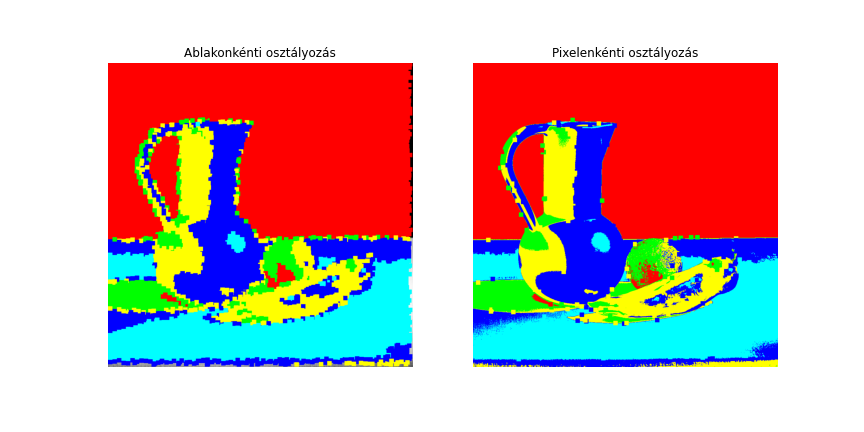
\includegraphics[scale=0.5]{images/window_pixel_segmentation.png}
\caption{Szegmentálás az \ref{method_window}. a illetve \ref{method_pixel}. módszerekkel.}
\label{fig:window_pixel_segmentation}
\end{figure}

Az \ref{method_window}. módszer egy olyan képet eredményez, ahol nincsenek lekerekített szélek, hanem átlógnak az ablakok egyik objektumból a másikba. A kép jobb szélén és az alján láthatóak szegmentálatlan részek, hiszen ha a címke nélküli pixel közelebb található a kép széléhez mint az ablak szélessége, akkor már nem tudunk ablakot készíteni hozzá, így nem is vizsgáljuk meg azokat a pontokat. Ezt a hibát ki lehetne úgy javítani, hogy külön ciklussal a címke nélküli pixeleket osztályozom ezeken a területeken. Ehhez a másik módszerben betanított modellt lehetne felhasználni.

Az eddigiekkel szemben a \ref{method_pixel}. módszer szegmentálása sokkal pontosabb, jobban elkülöníti az egymástól különböző szegmenseket. Itt nincsenek szegmentálatlan részek, minden pixel tartozik valahova.

Az tisztán látható, hogy mind a két módszer ugyanazokat a szegmenseket eredményezi. A futási idejüket tekintve amíg az \ref{method_window}. módszer pár másodperc alatt lefut, addig a \ref{method_pixel}. módszernek átlagban 14 perc szükséges a futásához.

Megvizsgáltam, hogy ha változtatom az ablakok méretét, akkor vajon sikerül-e jobb eredményt elérni a textúra alapú szegmentálás során. A vizsgálat eredménye a \ref{fig:window_different_px}. ábrán látható.

\begin{figure}[h]
\centering
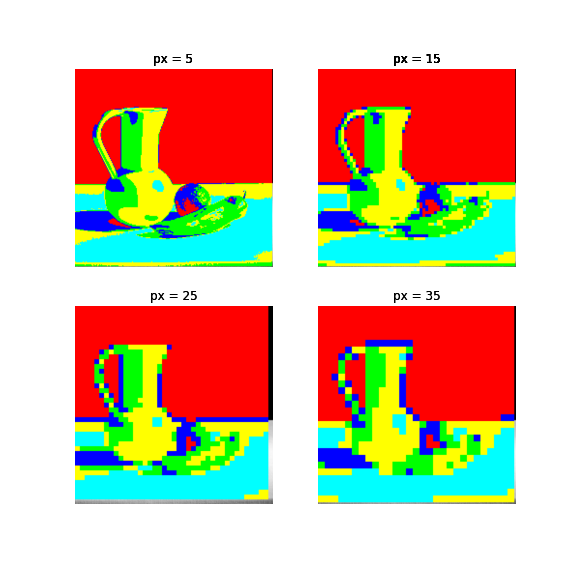
\includegraphics[scale=0.7]{images/window_different_px.png}
\caption{A kép szegmentálása különböző méretű ablakok segítségével.}
\label{fig:window_different_px}
\end{figure}

Azt feltételeznénk, hogy minél nagyobb az ablak, annál több információt tartalmaz, így valamivel pontosabb a szegmentálás. Ám jól látható, hogy hiába növeltem az ablakok méretét, az algoritmusom ugyan azokat a szegmenseket találta meg a képen. 

Mivel a kép szegmentálása megtörtént, így már csak a tényleges kiszínezése van hátra, amivel a következő fejezetben foglalkozok. 